\documentclass[11pt]{article}

\usepackage[margin=1in]{geometry}
\usepackage{amsmath,amssymb,amsthm}
\usepackage{booktabs}
\usepackage{graphicx}
\usepackage{hyperref}
\usepackage[numbers,sort&compress]{natbib}
\usepackage{enumitem}
\usepackage{microtype}

\hypersetup{
  colorlinks=true,
  linkcolor=blue,
  citecolor=blue,
  urlcolor=blue
}

\newtheorem{proposition}{Proposition}

\title{Task-Relevant Epiplexity:\\Separating Learnable Structure from Useful Structure}
\author{bossman-lab\\\texttt{bosis826@tutamail.com}}
\date{\today}

\begin{document}
\maketitle

\begin{abstract}
Epiplexity formalizes the structural information that a computationally bounded observer can extract from data. It offers a useful lens for understanding why likelihood training, synthetic data, data ordering, and emergent systems can produce reusable internal programs rather than mere memorization. However, task-agnostic structural information is not sufficient to explain transfer: a dataset may induce large amounts of structure while being irrelevant to a target task. We extend epiplexity in three ways. First, we define task-relevant epiplexity (TRE), the reduction in target task description length attributable to source-trained structure beyond matched controls. Second, we make the observer explicit through an observer specification covering architecture, optimizer, representation, ordering, context interface, inference protocol, and compute budget. Third, we introduce contextual epiplexity, the temporary structural information supplied by prompts, demonstrations, retrieval, and tool outputs at inference time. We provide two controlled experiments. A transparent PCA observer shows that total structure can be high while transfer remains at chance when the learned structure is target-irrelevant. A small next-token MLP experiment shows that learning-progress proxies can also decouple from transfer. These results do not claim to settle large-model behavior, but they motivate a stricter distinction between learnable structure and useful, transferable structure.
\end{abstract}

\section{Introduction}

Large models are often described as systems that learn from scale: more data, more parameters, and more compute. This description is true but incomplete. In practice, not all data of equal size has equal value. Data order, formatting, curriculum, synthetic generation, retrieval, and even a few in-context examples can change what a model learns or exhibits.

A natural explanation is that models do not merely store data. They build internal programs that compress and predict the data under finite compute. These programs may include syntax, algorithms, latent variables, world-model fragments, causal regularities, or reusable circuits. The recent notion of epiplexity \citep{finzi2026epiplexity} captures this intuition by measuring structural information available to a computationally bounded observer.

Yet a gap remains. Structural information is not the same as useful structural information. A music corpus, a cellular automaton, or a formal grammar can contain substantial learnable structure, but that structure may not help with legal reasoning, chess evaluation, or code execution. This creates a failure mode for strong proxy-based explanations of out-of-distribution performance \citep{li2026counterexample}: high structural complexity alone cannot guarantee transfer.

This paper proposes a more task-aware view. We argue that a theory of data value should answer three questions: (i) what structure can an observer extract from the data, (ii) which parts of that structure are relevant to a target task, and (iii) which parts can be made available at inference time through context, tools, or additional computation.

Our contributions are:
\begin{itemize}[leftmargin=*]
  \item We define an observer specification so epiplexity-like quantities are explicitly tied to model class, representation, ordering, inference protocol, and compute.
  \item We define task-relevant epiplexity as a target-conditioned reduction in description length beyond matched controls.
  \item We define contextual epiplexity as the inference-time analogue of structural information supplied by context.
  \item We provide two controlled experiments showing that total structure and learning progress can decouple from transfer.
\end{itemize}

\section{Background}

\subsection{Entropy, Compression, and Structure}

Shannon entropy measures average code length under a distribution. It captures unpredictability, but not whether that unpredictability contains learnable structure. A random string can have high entropy and little reusable structure. A short algorithmic text can have lower entropy yet induce reusable mechanisms in a learner.

Kolmogorov complexity measures the length of the shortest program that generates an object. It connects compression and programs, but its classical form assumes unbounded computation. Under unbounded compute, many complex phenomena have short descriptions: chess rules, cellular automata, and physical dynamics may be compactly specified even though their useful predictive abstractions are difficult to obtain.

The minimum description length (MDL) principle \citep{rissanen2004mdl,grunwald2007mdl} combines model cost and data cost. A useful model is worth encoding when it reduces the residual cost of the data. Epiplexity can be understood as a time-bounded MDL decomposition: the model part captures structural information, and the residual code length captures time-bounded randomness. This view is compatible with compression interpretations of language modeling \citep{deletang2023compression}.

\subsection{Epiplexity}

Let an observer be restricted to probabilistic programs that run within a time budget $T$. For a random variable $X$, the time-bounded MDL objective selects a program $P^\star$ minimizing
\begin{equation}
  |P| + \mathbb{E}[-\log P(X)].
\end{equation}
The epiplexity $S_T(X)$ is the description length $|P^\star|$; the time-bounded entropy $H_T(X)$ is the residual expected code length $\mathbb{E}[-\log P^\star(X)]$. Intuitively, epiplexity measures the structural information that must be stored in the model to explain the data under the compute budget.

This perspective helps explain why deterministic computation can create information for bounded observers, why data order matters, and why likelihood training may induce predictive structures that were not explicit in the generating process.

\subsection{The Missing Distinction}

Epiplexity is a measure of extractable structure. Transfer requires more: the extracted structure must be relevant to the target. A strong form of the claim ``higher epiplexity implies better OOD performance'' is false in general. The same issue applies to many proxies: held-out loss, compression ratio, learning progress, or representation complexity can fail when the learned structure is unrelated to the downstream task.

\section{Observer Specification}

We define an observer specification
\begin{equation}
  \Omega = (A, M, \tau, O, C, I, T),
\end{equation}
where $A$ is the training algorithm and optimizer, $M$ is the model family, $\tau$ is the representation or tokenization, $O$ is the data ordering and conditioning protocol, $C$ is the context interface, $I$ is the inference protocol, and $T$ is the training and inference compute budget.

We then write $S_\Omega(X)$ for the structural information extractable from data $X$ by observer $\Omega$. This notation is deliberately less elegant than $S_T(X)$, but it is more faithful to engineering reality. The same data can expose different structure to different architectures, tokenizers, orderings, and context protocols.

\section{Task-Relevant Epiplexity}

Let $X$ be source data and $Z=(U,V)$ be a target task with inputs $U$ and outputs $V$. Let $\theta_X$ be the state, weights, or encoded program produced by training observer $\Omega$ on $X$.

Define the target transfer gain
\begin{equation}
  \Delta_\Omega(X \rightarrow Z)
  = L_\Omega(Z) - L_\Omega(Z \mid \theta_X),
\end{equation}
where $L_\Omega(Z)$ is the description length of the target task without the source-trained state, and $L_\Omega(Z \mid \theta_X)$ is the description length when the source-trained state is available. This conditional code must include any adapter, probe, prompt, or fine-tuning cost required to use $\theta_X$.

To avoid confusing leakage, surface statistics, or generic complexity with target relevance, we introduce matched controls. Let $\mathcal{C}(X)$ be a set of control sources that preserve non-target properties of $X$ such as length distribution, token frequencies, local statistics, or total structure, while disrupting the target-relevant relationship.

We define task-relevant epiplexity
\begin{equation}
  \mathrm{TRE}_\Omega(X;Z)
  =
  \Delta_\Omega(X \rightarrow Z)
  -
  \mathbb{E}_{X' \in \mathcal{C}(X)}
  \Delta_\Omega(X' \rightarrow Z).
\end{equation}
This quantity separates two claims: $S_\Omega(X)$ is high means the observer learned much structure; $\mathrm{TRE}_\Omega(X;Z)$ is high means the observer learned structure useful for $Z$.

\begin{proposition}[High structure does not imply high TRE]
There exist source data distributions $X_1, X_2$ and a target task $Z$ such that
\begin{equation}
  S_\Omega(X_1) > S_\Omega(X_2)
  \quad\text{but}\quad
  \mathrm{TRE}_\Omega(X_1;Z) < \mathrm{TRE}_\Omega(X_2;Z).
\end{equation}
\end{proposition}
\begin{proof}[Proof sketch]
Let the observer learn a high-dimensional structured subspace unrelated to $Z$ from $X_1$, and a lower-dimensional subspace aligned with $Z$ from $X_2$. The first source has higher extractable structure, but only the second reduces the target code length. The PCA experiment in Section~\ref{sec:pca} instantiates this construction.
\end{proof}

\section{Contextual Epiplexity}

Inference-time context can change what a model is able to do without changing its weights. Few-shot examples \citep{brown2020fewshot}, retrieved evidence, intermediate reasoning, and tool outputs can expose latent variables, specify a data format, or reduce a search space. Mechanistic work on induction heads gives one concrete family of circuits for context-sensitive behavior \citep{olsson2022induction}.

For query $Q$, answer $Y$, and context $K$, define
\begin{equation}
  \mathrm{CE}_\Omega(K;Y \mid Q)
  =
  L_\Omega(Y \mid Q) - L_\Omega(Y \mid Q,K).
\end{equation}
This contextual epiplexity measures how much the context reduces the description length of the answer. A controlled version subtracts matched contexts:
\begin{equation}
  \mathrm{CRE}_\Omega(K;Y \mid Q)
  =
  \mathrm{CE}_\Omega(K;Y \mid Q)
  -
  \mathbb{E}_{K' \in \mathcal{C}(K)}
  \mathrm{CE}_\Omega(K';Y \mid Q).
\end{equation}
Examples of control contexts include label-shuffled demonstrations, same-topic but irrelevant retrieval, format-preserving explanations with broken causal steps, or tool outputs with corrupted values \citep{zhao2021calibrate}.

\section{Predictions}

The framework makes several falsifiable predictions:
\begin{itemize}[leftmargin=*]
  \item Total structure can be high while transfer is low.
  \item Task-relevant structure should predict transfer better than total structure when controls are matched.
  \item Data ordering affects transfer through the structures it makes accessible to the observer.
  \item In-context examples improve performance when they supply task-relevant temporary structure, not merely when they add format or length.
  \item Learning-progress proxies can fail when progress is driven by target-irrelevant regularities.
\end{itemize}
If task-relevant epiplexity does not outperform loss, loss slope, total structure, or representation probes under controlled interventions, then the framework should be weakened.

\section{Experiment 1: PCA Observer}
\label{sec:pca}

\subsection{Setup}

We construct a transparent observer: PCA followed by a few-shot ridge classifier. Inputs have dimension 32. The downstream target depends only on the last four coordinates. The source data varies in whether its dominant structure is target-relevant: \texttt{random}, \texttt{irrelevant\_high}, \texttt{relevant\_mid}, \texttt{mixed\_budget\_limited}, and \texttt{relevant\_high}. The PCA observer learns $k$ components from source data. We then freeze the PCA representation and train a ridge classifier on 24 labeled target examples.

We report total-structure proxy, target alignment, a TRE proxy, and transfer accuracy. Full details and scripts are in Appendix~\ref{app:repro}.

\begin{figure}[t]
  \centering
  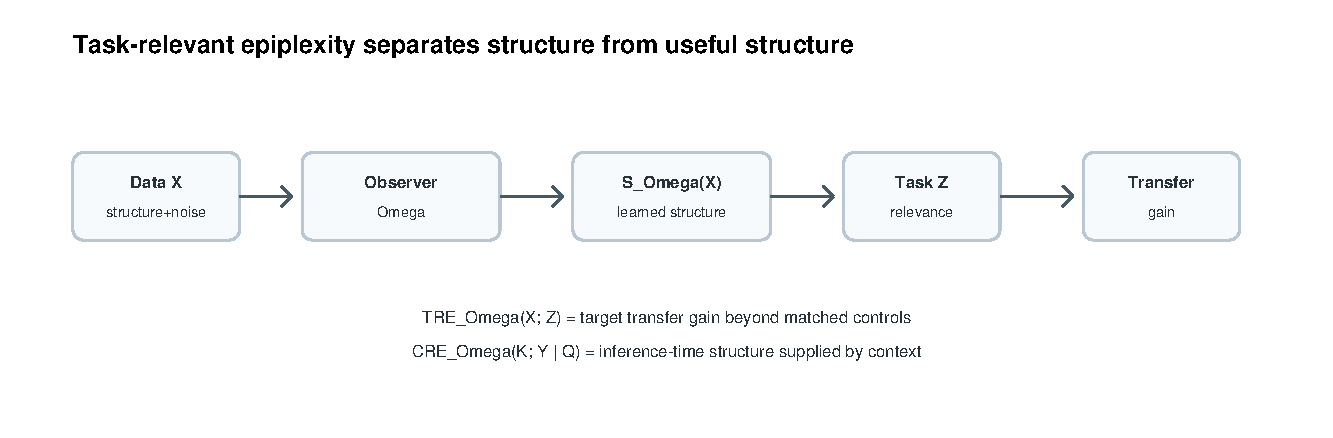
\includegraphics[width=0.95\linewidth]{figures/framework_diagram.pdf}
  \caption{Framework overview. Total extractable structure is not the same as task-relevant structure. TRE measures target transfer gain beyond matched controls, and contextual epiplexity extends the idea to inference-time information.}
  \label{fig:framework}
\end{figure}

\begin{table}[t]
  \centering
  \small
  \caption{PCA observer results for $k=4$. Total structure can be high while transfer remains at chance if the learned subspace is target-irrelevant.}
  \label{tab:pca}
  \begin{tabular}{lrrrr}
    \toprule
    Source & Total structure & Alignment & TRE proxy & Transfer acc. \\
    \midrule
    random & $0.4755$ & $0.1258$ & $0.0602$ & $0.5444$ \\
    irrelevant\_high & $22.0220$ & $0.0001$ & $0.0024$ & $0.5006$ \\
    relevant\_mid & $7.0369$ & $0.9967$ & $7.0137$ & $0.8100$ \\
    mixed\_budget\_limited & $21.0801$ & $0.0006$ & $0.0120$ & $0.5022$ \\
    relevant\_high & $24.5222$ & $0.9993$ & $24.5048$ & $0.8120$ \\
    \bottomrule
  \end{tabular}
\end{table}

\subsection{Results}

At $k=4$, \texttt{irrelevant\_high} has total structure $22.0220 \pm 0.2044$, far higher than \texttt{relevant\_mid} at $7.0369 \pm 0.1126$. Yet \texttt{irrelevant\_high} transfer is $0.5006 \pm 0.0079$, while \texttt{relevant\_mid} transfer is $0.8100 \pm 0.0401$.

Across all runs, the Pearson correlation between total structure and transfer is $-0.0252$. The correlation between target alignment and transfer is $0.9086$. The correlation between the TRE proxy and transfer is $0.6004$, with Spearman correlation $0.7230$.

\begin{figure}[t]
  \centering
  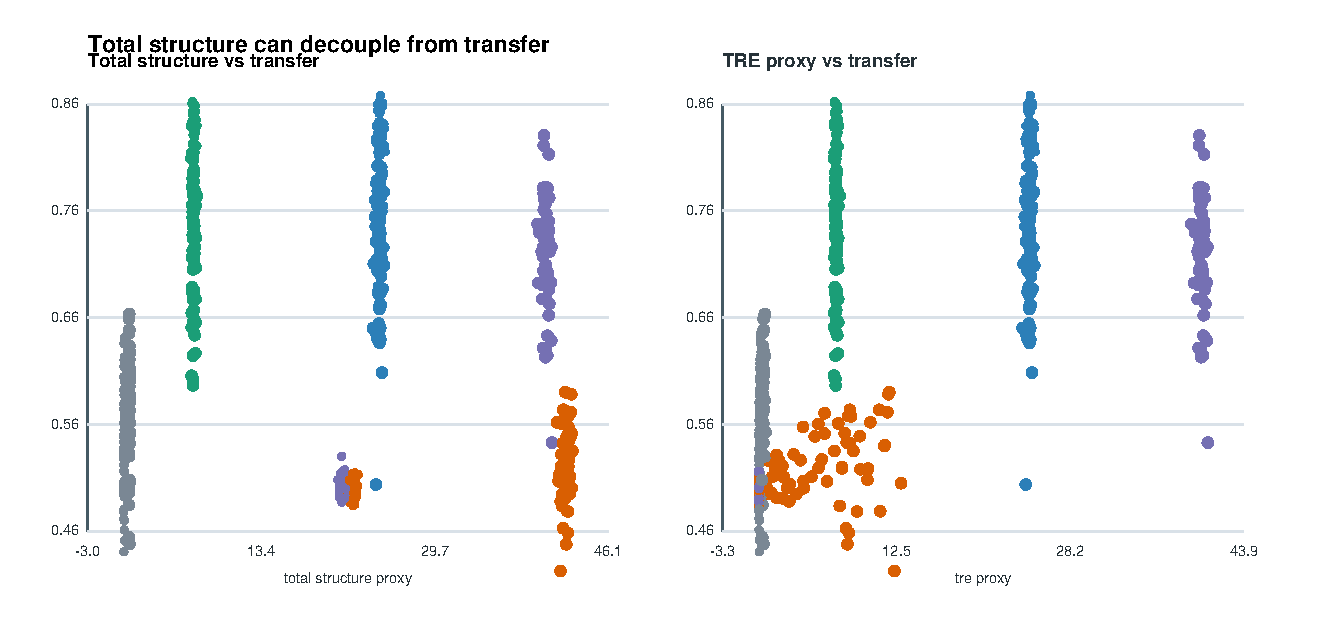
\includegraphics[width=0.95\linewidth]{figures/pca_metric_scatter.pdf}
  \caption{PCA experiment. Total structure alone is not predictive of transfer, while target-aware structure is more aligned with transfer.}
  \label{fig:pca-scatter}
\end{figure}

The mixed source illustrates observer dependence. With $k=4$, the observer spends capacity on irrelevant high-variance structure and transfers at chance. With $k=12$, the target-relevant subspace becomes visible, target alignment rises to $0.9975 \pm 0.0010$, and transfer accuracy rises to $0.7212 \pm 0.0514$.

\begin{figure}[t]
  \centering
  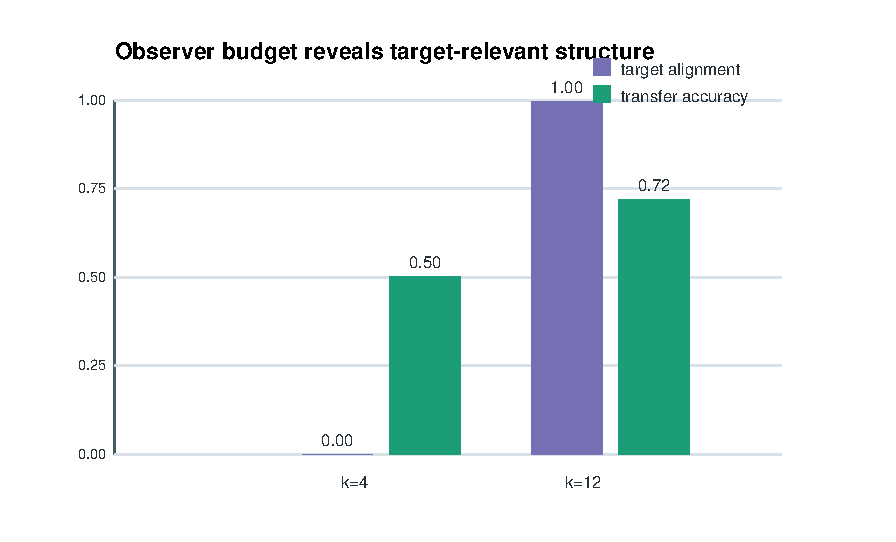
\includegraphics[width=0.68\linewidth]{figures/pca_budget_effect.pdf}
  \caption{Observer budget matters. The same mixed source is unhelpful when the representation budget misses the target-relevant subspace, but useful when the observer can include it.}
  \label{fig:pca-budget}
\end{figure}

\section{Experiment 2: Next-Token MLP}

\subsection{Setup}

The PCA experiment is transparent but not language-model-like. We therefore implement a second controlled experiment using a one-hidden-layer MLP trained for next-token prediction on synthetic binary sequences. After training, the hidden representation is frozen and used by a few-shot ridge classifier for a target recurrence task.

Source distributions are \texttt{random}, \texttt{irrelevant\_rule}, \texttt{relevant\_rule}, and \texttt{mixed\_rule}. The learning-progress proxy is the area of the validation loss curve above the final loss.

\begin{table}[t]
  \centering
  \small
  \caption{Next-token MLP experiment. Learning progress can be driven by target-irrelevant regularities.}
  \label{tab:sequence}
  \begin{tabular}{lrrrr}
    \toprule
    Source & Final loss & Learning progress & Loss reduction & Transfer acc. \\
    \midrule
    random & $0.6933$ & $0.0115$ & $0.0051$ & $0.5277$ \\
    irrelevant\_rule & $0.5855$ & $1.5835$ & $0.1126$ & $0.5380$ \\
    relevant\_rule & $0.2599$ & $0.4760$ & $0.2272$ & $0.5685$ \\
    mixed\_rule & $0.6399$ & $0.7811$ & $0.0591$ & $0.5859$ \\
    \bottomrule
  \end{tabular}
\end{table}

\subsection{Results}

The \texttt{irrelevant\_rule} source has learning progress $1.5835 \pm 1.5587$, higher than \texttt{relevant\_rule} at $0.4760 \pm 0.1213$, but its transfer accuracy is lower: $0.5380 \pm 0.1105$ versus $0.5685 \pm 0.0865$. Across all runs, learning progress has Pearson correlation $-0.1084$ with transfer, and loss reduction has Pearson correlation $-0.0162$.

\begin{figure}[t]
  \centering
  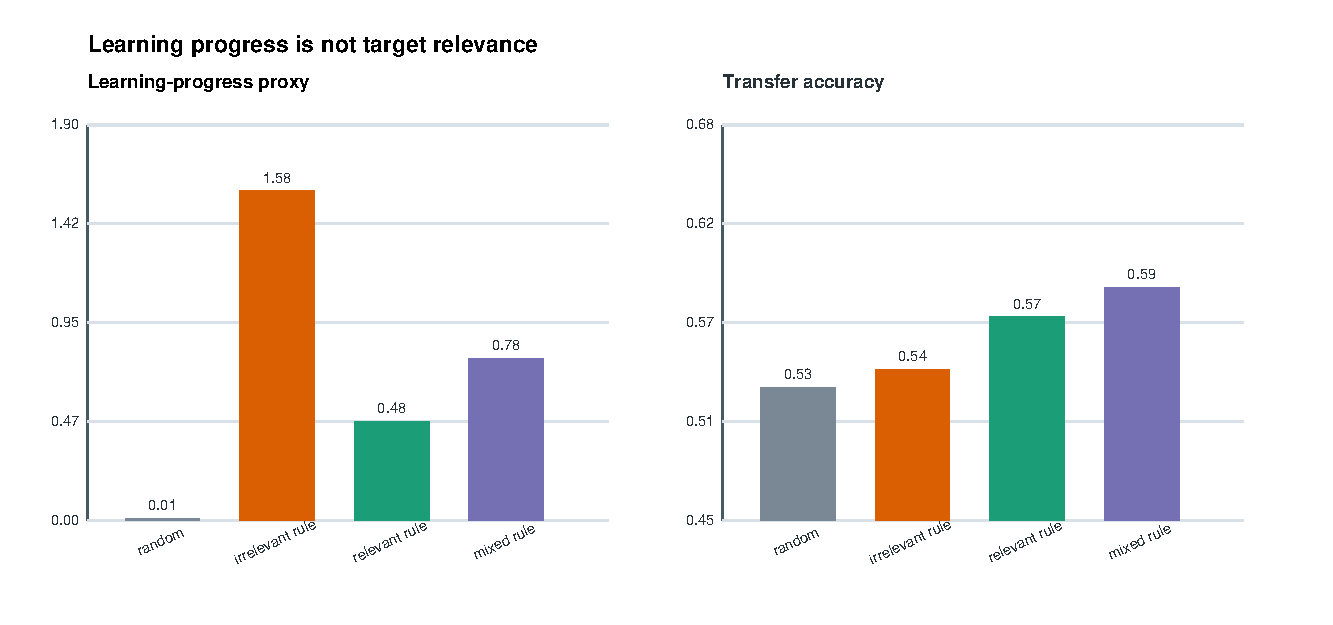
\includegraphics[width=0.95\linewidth]{figures/sequence_mlp_bars.pdf}
  \caption{Next-token MLP experiment. The source with the largest learning-progress proxy is not the one with the best target transfer.}
  \label{fig:sequence}
\end{figure}

This result is weaker and noisier than the PCA experiment, but it adds a next-token training dynamic: simply being learnable by an autoregressive model does not imply usefulness for the target task.

\section{Related Work}

This work builds on epiplexity and computationally bounded information measures \citep{finzi2026epiplexity}, MDL and prequential coding \citep{rissanen2004mdl,grunwald2007mdl}, compression views of language modeling \citep{deletang2023compression}, and work on in-context learning and induction heads \citep{brown2020fewshot,olsson2022induction}. It is also related to representation learning, transfer learning, data selection, curriculum learning, information bottleneck methods, and recent counterexamples to strong proxy-based explanations of OOD performance \citep{li2026counterexample}.

The key distinction is that we do not propose a new task-agnostic universal data value. Instead, we separate task-agnostic structure from target-relevant structure and make the observer explicit.

\section{Limitations}

The experiments are controlled and small. They do not establish large-model scaling behavior. The PCA observer is intentionally simple; the MLP observer is closer to language modeling but still far from modern transformers.

TRE is target-dependent. This is a limitation if one wants a single universal data value, but it is necessary for explaining transfer to a specified target family.

The definition depends on controls. Poorly chosen controls can hide or exaggerate target relevance. A practical theory of TRE requires careful matched-control design.

The conditional code $L_\Omega(Z \mid \theta_X)$ must account for adapters, probes, prompts, or fine-tuning. If these costs are ignored, TRE may collapse into downstream performance.

Finally, contextual epiplexity remains conceptual in this draft. It requires dedicated experiments with label-shuffled demonstrations, corrupted retrieval, and tool-output controls.

\section{Conclusion}

Epiplexity reframes learning as the extraction of structural information by a computationally bounded observer. We argue that a theory of transfer must go one step further: it must separate structure from useful structure.

Task-relevant epiplexity measures whether source-trained structure reduces the description length of a target task beyond matched controls. Observer specification makes the quantity reproducible and architecture-aware. Contextual epiplexity extends the same idea to inference-time information supplied by prompts, retrieval, demonstrations, and tools.

The resulting picture is that observed intelligence combines stored structure in parameters, task-relevant reusable structure, temporary structure in context, and inference-time compute and tools. This is not a complete theory of intelligence. It is a proposal for making one important distinction measurable: the distinction between data that a model can learn from and data that helps it solve the tasks we care about.

\appendix

\section{Reproducibility}
\label{app:repro}

The experiments can be reproduced with:
\begin{verbatim}
.\run_all_experiments.ps1
\end{verbatim}
or manually:
\begin{verbatim}
python experiments\task_relevant_epiplexity_pca.py
python experiments\analyze_pca_results.py
python experiments\sequence_mlp_transfer.py
python experiments\analyze_sequence_results.py
python experiments\export_paper_figures.py
\end{verbatim}

The generated outputs are stored under \texttt{experiments/results}, \texttt{experiments/figures}, and \texttt{paper/figures}. The experiments use fixed random seeds and require only NumPy, pandas, and reportlab.

\section{Figure Sources}

The PDF figures in this manuscript are generated from the CSV result files. The corresponding SVG quick-view versions are:
\begin{itemize}[leftmargin=*]
  \item \texttt{experiments/figures/framework\_diagram.svg}
  \item \texttt{experiments/figures/pca\_metric\_scatter.svg}
  \item \texttt{experiments/figures/pca\_budget\_effect.svg}
  \item \texttt{experiments/figures/sequence\_mlp\_bars.svg}
\end{itemize}

\bibliographystyle{plainnat}
\bibliography{references}

\end{document}
